\documentclass[a4paper,11pt,exos]{nsi} % COMPILE WITH DRAFT


%\pagestyle{empty}
\begin{document}

\setlength{\columnseprule}{0pt}
\setlength{\columnsep}{1cm}

\classe{\premiere spe}
\titre{Trigonométrie}
\maketitle


\subsection*{Mesurer un angle en radians}

\exo{}
Dire si chacune des affirmations suivantes et vraie ou fausse. Justifier lorsque c'est faux.
\begin{enumerate}
	\item 	Lors de l'enroulement de la droite numérique, les points images des nombres réels positifs se situent au-dessus de l'axe des abscisses.
	\item 	À chaque nombre réel correspond un unique point image sur le cercle trigonométrique.
	\item	À chaque point du cercle trigonométrique correspond un unique réel de la droite numérique.
	\item	Le nombre 3 n'a pas d'image sur le cercle trigonométrique. 
\end{enumerate}


\begin{minipage}{12cm}
	\exo{}
	Pour chacun des réels suivant, donner le quadran dans lequel il se trouvera lors de l'enroulement de la droite numérique.
	\begin{multicols}{2}
		\begin{enumerate}
			\item 	$\dfrac{2\pi}{3}$
			\item 	$\dfrac{\pi}{8}$
			\item	$\dfrac{5\pi}{4}$
			\item	$\dfrac{-2\pi}{3}$
		\end{enumerate}
	\end{multicols}
	
\end{minipage}
\begin{minipage}{5cm}
	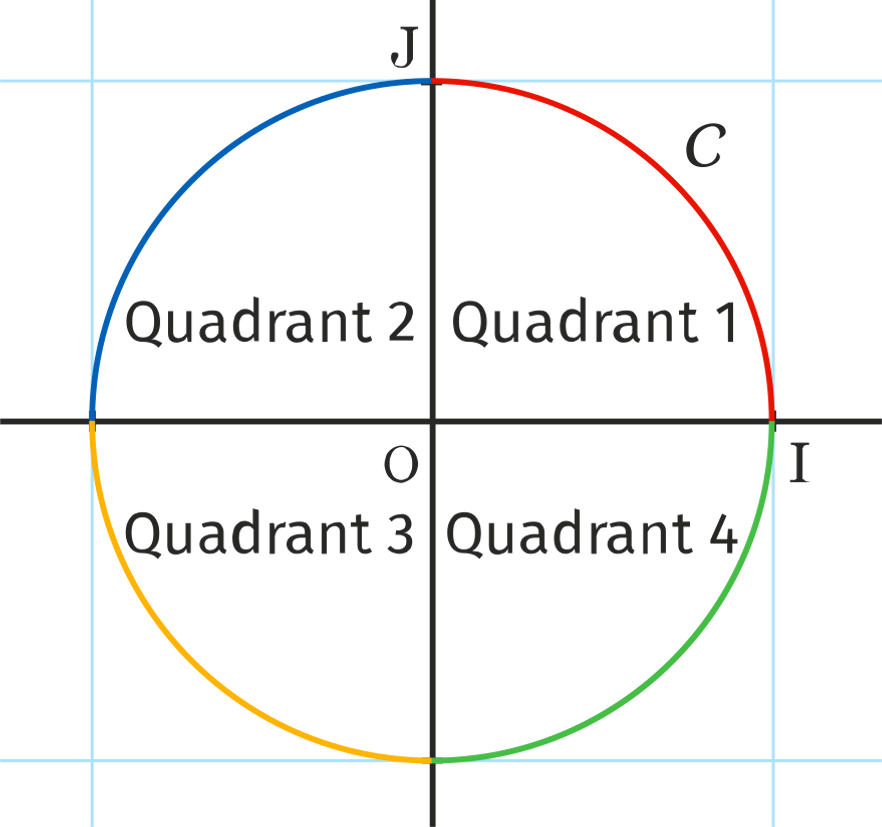
\includegraphics[width=5cm]{quadrants}
\end{minipage}


\exo{}
Dans chacune des listes suivantes, il y a un intrus. Le trouver en justifiant.
\begin{multicols}{2}
    \begin{enumerate}
        \item 	$\dfrac{3\pi}{2}\ ; \quad\dfrac{9\pi}{2}\ ;\quad \dfrac{-\pi}{2}\ ;\quad \dfrac{-5\pi}{2}$.
        \item 	$\dfrac{\pi}{3}\ ; \quad\dfrac{14\pi}{3}\ ;\quad \dfrac{-8\pi}{6}\ ;\quad \dfrac{-10\pi}{3}$.
        \item	$\dfrac{7\pi}{4}\ ; \quad\dfrac{-\pi}{4}\ ;\quad \dfrac{-9\pi}{4}\ ;\quad \dfrac{-19\pi}{4}$.
        \item	$\pi\ ;\quad -\pi\ ;\quad \pi\sqrt{9}\ ;\quad 0$.
    \end{enumerate}
    
\end{multicols}



\exo{}
\begin{minipage}{8cm}
	Sur les figures ci-contre, $ABCD$ est un carré, BCE est un triangle équilatéral et FHG est un triangle isocèle en F. De plus, on sait que $\widehat{HFG}=\dfrac{\pi}{5}$.\\[1em]
	Déterminer les valeurs en radian des angles $\widehat{FHG}, \widehat{BEC}$ et $\widehat{ABE}$.
\end{minipage}
\begin{minipage}{9cm}
	\flushright 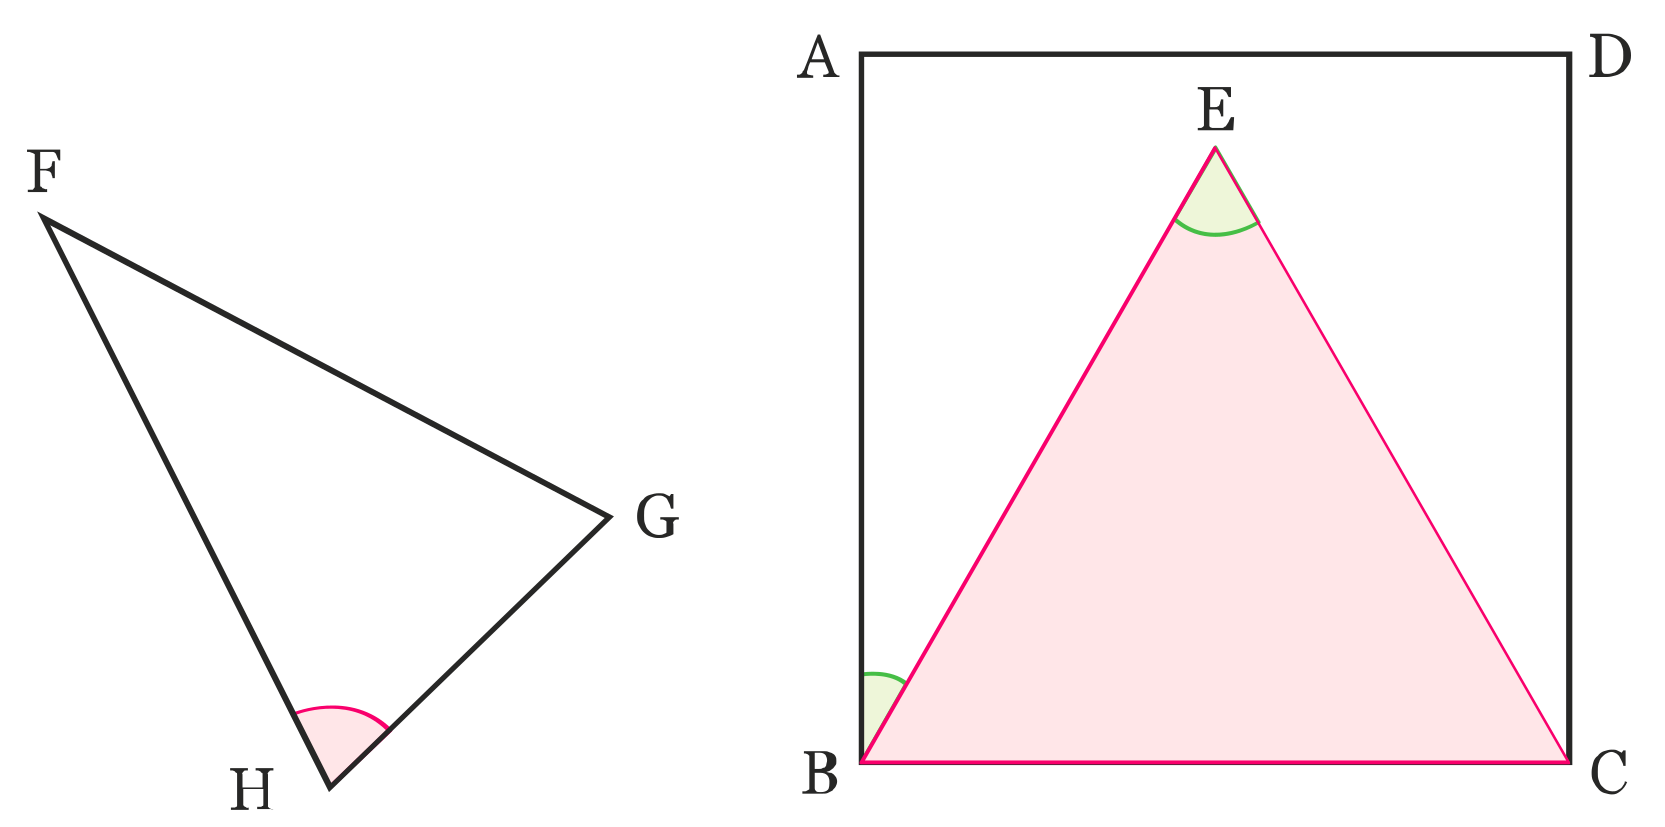
\includegraphics[width=8.5cm]{figure1}
\end{minipage}
\vspace{1cm}


\begin{minipage}{10cm}
	\exo{}
	On considère le cercle trigonométrique ci-dessous dans lequel est inscrit un pentagone régulier $IBCDE$.\\[1em]
	Donner, pour chaque sommet du pentagone, un réel qui lui est associé.
\end{minipage}
\begin{minipage}{7cm}
	\flushright 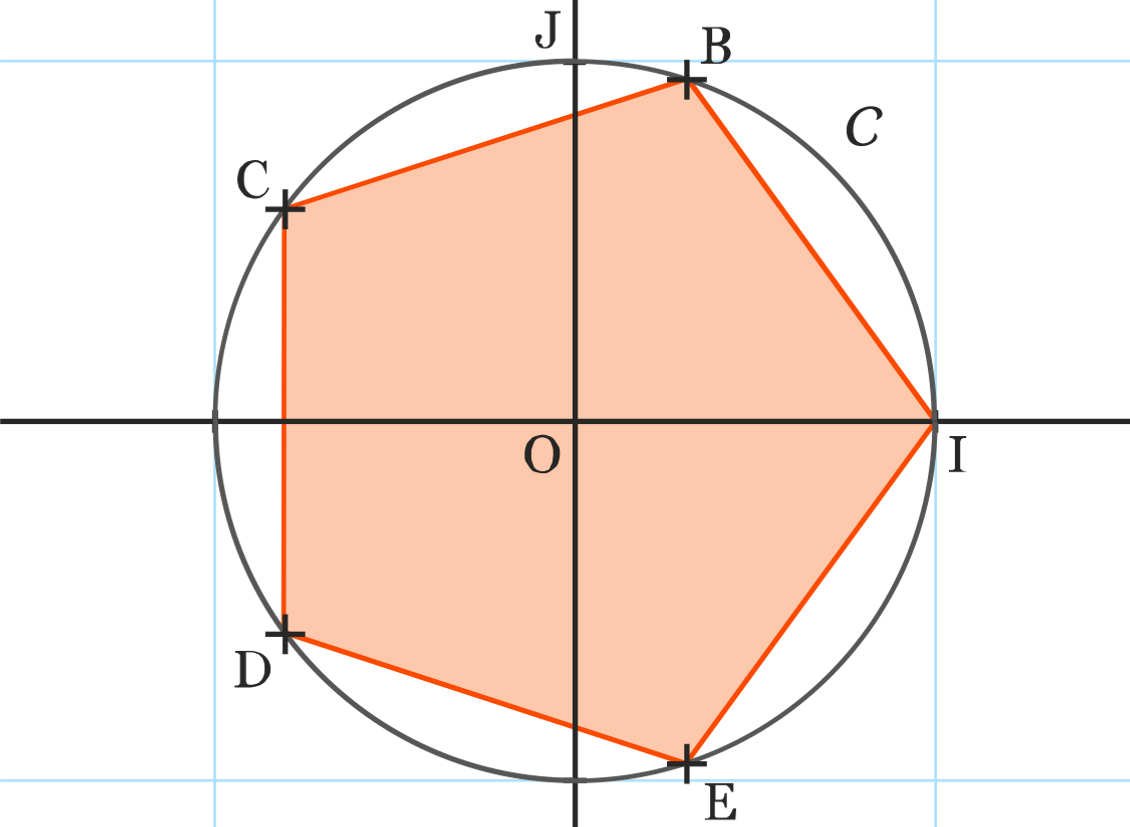
\includegraphics[width=6.5cm]{pentagone}
\end{minipage}



\exo{}
Compléter le tableau des mesures d'angles suivant. On arrondira les mesures en degré à l'unité.
\begin{center}
	\renewcommand{\arraystretch}{2.4}
	\begin{tabular}{|c|c|c|c|c|c|}
		\hline 
		Mesure d'angle en degrés & $\quad 20\quad $&$\quad 168\quad$ &$\quad \quad $&$\quad \quad$ &$\quad 245\quad$  \\ 
		\hline 
		Mesure d'angle en radians &  &  & $\quad\dfrac{\pi}{7}\quad$ & $\quad\dfrac{\pi}{13}\quad$ &  \\ 
		\hline 
	\end{tabular} 
\end{center}


\exo{}
Un angle de $\dfrac{\pi}{6}$ radian correspond à un angle de 30°.\\[.5em]
Sans calculatrice, en déduire a mesure en radian des angles suivants.
\begin{multicols}{4}
	\begin{enumerate}
		\item 	3°
		\item 	15°
		\item	37,5°
		\item	120°	
	\end{enumerate}
\end{multicols}

\subsection*{Cosinus et sinus d'un nombre réel}

\exo{}
\begin{minipage}{12cm}
	On considère le cercle trigonométrique ci-contre.\\
	$M$ est le point image sur le cercle d'un nombre réel $x$. Compléter le tableau suivant avec le signe de $\cos(x)$ et $\sin(x)$ en fonction de la position du point $M$ sur le cercle.
	\begin{center}
		\begin{tabular}{|c|c|c|c|c|}
			\hline
			\cellcolor{UGLiOrange}$M$ est dans le quadrant & 1 & 2 & 3 & 4\\
			\hline
			\cellcolor{UGLiOrange}Signe de $\cos(x)$ & \hspace{1cm} & \hspace{1cm} & \hspace{1cm} & \hspace{1cm} \\
			\hline
			\cellcolor{UGLiOrange}Signe de $\sin(x)$ & \hspace{1cm} & \hspace{1cm} & \hspace{1cm} & \hspace{1cm} \\
			\hline
		\end{tabular}
	\end{center}
\end{minipage}
\begin{minipage}{5cm}
	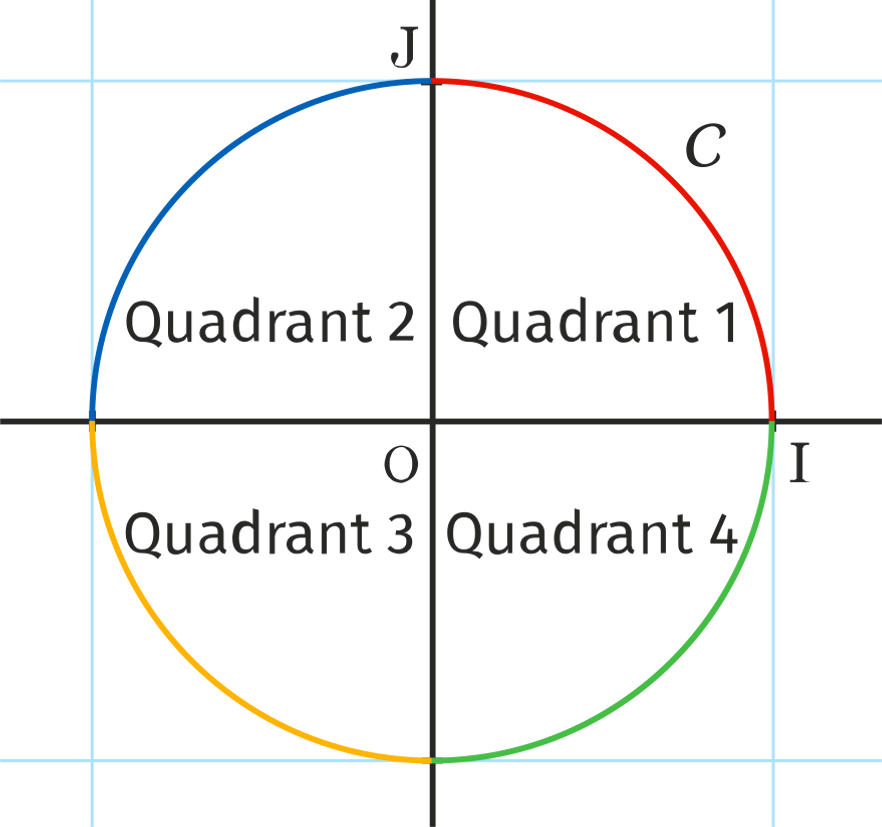
\includegraphics[width=5cm]{quadrants}
\end{minipage}




\begin{minipage}{8.5cm}
	\exo{}
	En utilisant le cercle trigonométrique ci-contre, compléter le tableau suivant.
	\begin{center}
		\renewcommand{\arraystretch}{2}
		\begin{tabular}{|c|c|c|c|c|c|}
			\hline
			\cellcolor{UGLiOrange} $x$ & $\dfrac{2\pi}{3}$ & $\dfrac{3\pi}{4}$ & $\dfrac{-5\pi}{6}$ & $\dfrac{-3\pi}{4}$ & $\dfrac{-\pi}{2}$ \\
			\hline
			\cellcolor{UGLiOrange} Point image & \hspace{.7cm} & \hspace{.7cm} & \hspace{.7cm} & \hspace{.7cm} & \hspace{.7cm} \\
			\hline
			\cellcolor{UGLiOrange} $\cos(x)$ & & & & & \\
			\hline
			\cellcolor{UGLiOrange} $\sin(x)$ & & & & & \\
			\hline
		\end{tabular}
	\end{center}
\end{minipage}
\begin{minipage}{8.5cm}
	\flushright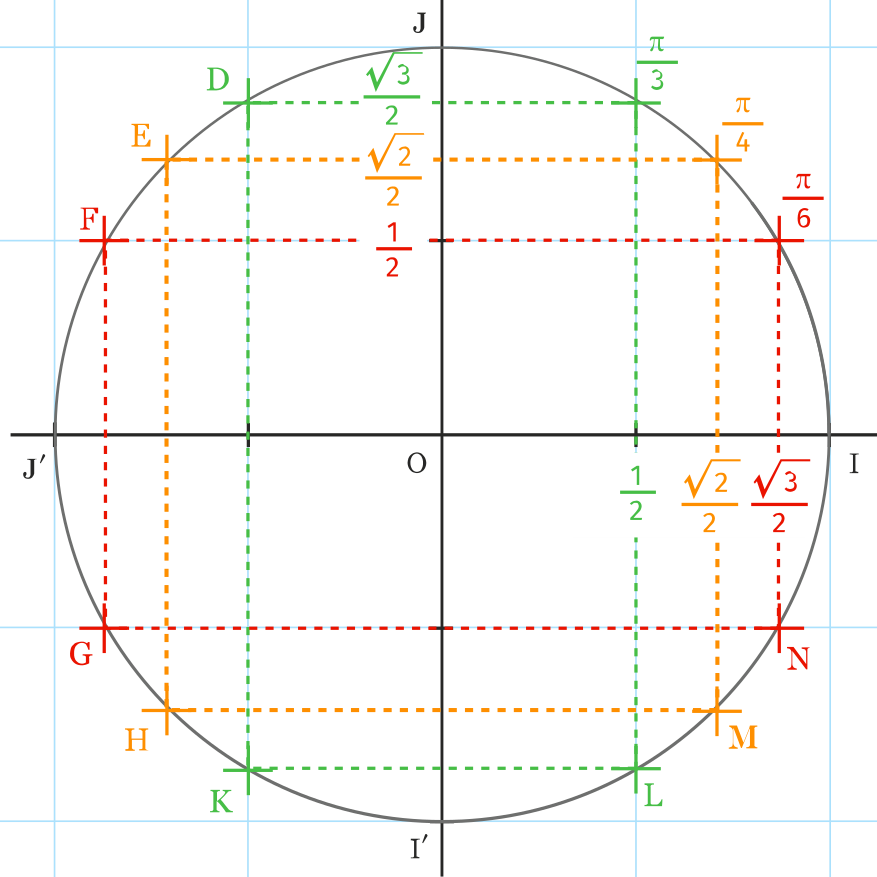
\includegraphics[width=8.2cm]{cercletrigo}
\end{minipage}
%\vspace{.5cm}


\exo{}
Sans calculatrice, calculer et réduire au même dénominateur les expressions suivantes.\\
Indiquer les étapes intermédiaires.
\begin{multicols}{2}
	\begin{enumerate}
		\item 	$\cos\left(\dfrac{-\pi}{3}\right)-\sin\left(\dfrac{-7\pi}{4}\right)$
		\item 	$\cos\left(\dfrac{5\pi}{3}\right)-\sin\left(2\pi\right)+\cos\left(\dfrac{-\pi}{6}\right)$	
		\item	$\sin\left(-2022\pi\right)-\cos\left(\dfrac{-\pi}{4}\right)+\sin\left(\dfrac{3\pi}{2}\right)-\sin\left(\dfrac{\pi}{4}\right)$
		\item	$\cos\left(\dfrac{\pi}{6}\right)+\sin\left(\dfrac{\pi}{3}\right)-\sin\left(\dfrac{\pi}{2}\right)+\sin\left(\dfrac{4\pi}{3}\right)$
	\end{enumerate}
\end{multicols}


\exo{}
Sans calculatrice, calculer les expressions suivantes.\\
Indiquer les expressions intermédiaires s'il y en a.
\begin{multicols}{2}
	\begin{enumerate}
		\item 	$\cos^2\left(\dfrac{-\pi}{13}\right)+\sin^2\left(\dfrac{-\pi}{13}\right)$
		\item 	$\cos^2\left(\dfrac{-\pi}{6}\right)	-\sin^2\left(\dfrac{-\pi}{6}\right)$
		\item	$\sin\left(\dfrac{-5\pi}{6}\right)\times \cos\left(\dfrac{2\pi}{3}\right)-\cos(-\pi)$
		\item	$\dfrac{\sin\left(\dfrac{\pi}{4}\right)}{\cos^2\left(\dfrac{\pi}{3}\right)}$
	\end{enumerate}
\end{multicols}



\exo{}
On note $\tan(x)$ le quotient de $\sin(x)$ par $\cos(x)$, défini pour tout $x$ tel que $\cos(x)\neq0$.\\
Par exemple, $\quad \tan(\pi)=\dfrac{\sin(\pi)}{\cos(\pi)}=\dfrac{0}{-1}=0$.\\[.5em]
Compléter, lorsque c'est possible, le tableau suivant.
\begin{center}
	\renewcommand{\arraystretch}{2}
	\begin{tabular}{|c|c|c|c|c|c|c|}
		\hline
		\cellcolor{UGLiOrange}$x$ & $0$ & $\dfrac{\pi}{3}$ & $\dfrac{\pi}{4}$ & $-\dfrac{\pi}{6}$ & $3\pi$ & $\dfrac{\pi}{2}$ \\
		\hline
		\cellcolor{UGLiOrange} $\tan(x)$ & \hspace{1cm} & \hspace{1cm} & \hspace{1cm} & \hspace{1cm} & \hspace{1cm} & \hspace{1cm} \\
		\hline
	\end{tabular}
\end{center}
\vspace{.5cm}

\exo{}
la tangente d'un réel $x$ est définie par $\tan(x)=\dfrac{\sin(x)}{\cos(x)}$ pour toutes les valeurs de $x\in\mathcal{D}_T$ où $\cos(x)\neq0$.\\
Montrer que pour tous les réels $x\in \mathcal{D}_T$, on a : $\quad\tan^2(x)=\dfrac{1}{\cos^2(x)}-1$.



\exo{}
Dans chacun des cas suivants, déterminer un nombre réel $x$ vérifiant les conditions données.
\begin{multicols}{2}
	\begin{enumerate}
		\item 	$\cos(x)=\dfrac{-\sqrt{2}}{2}$
			\begin{enumalph}
				\item 	avec $x\in\fio{0}{\pi}$
				\item 	avec $x\in\oif{-\pi}{-\dfrac{\pi}{2}}	$
			\end{enumalph}
		\item 	$\sin(x)=\dfrac{1}{2}$
		\begin{enumalph}
			\item 	avec $x\in\fio{\dfrac{\pi}{2}}{\pi}$
			\item 	avec $x\in\fio{-\dfrac{\pi}{2}}{\dfrac{\pi}{2}}$
		\end{enumalph}
	\end{enumerate}
\end{multicols}




\begin{minipage}{9cm}
	\exo{}
	Des ingénieurs de l'Office national des forêts veulent estimer la hauteur d'un pin en plaçant leur tachéomètre au point $O$. Ils ont relevé les données suivantes :
	$$OA=15 \text{m}, \quad \widehat{SOA}=45°\quad \text{et}\quad \widehat{AOP}=30°$$
	Calculer la hauteur $h$ de l'arbre (donner la valeur exacte et un arrondi au décimètre.)
\end{minipage}
\begin{minipage}{8cm}
	\flushright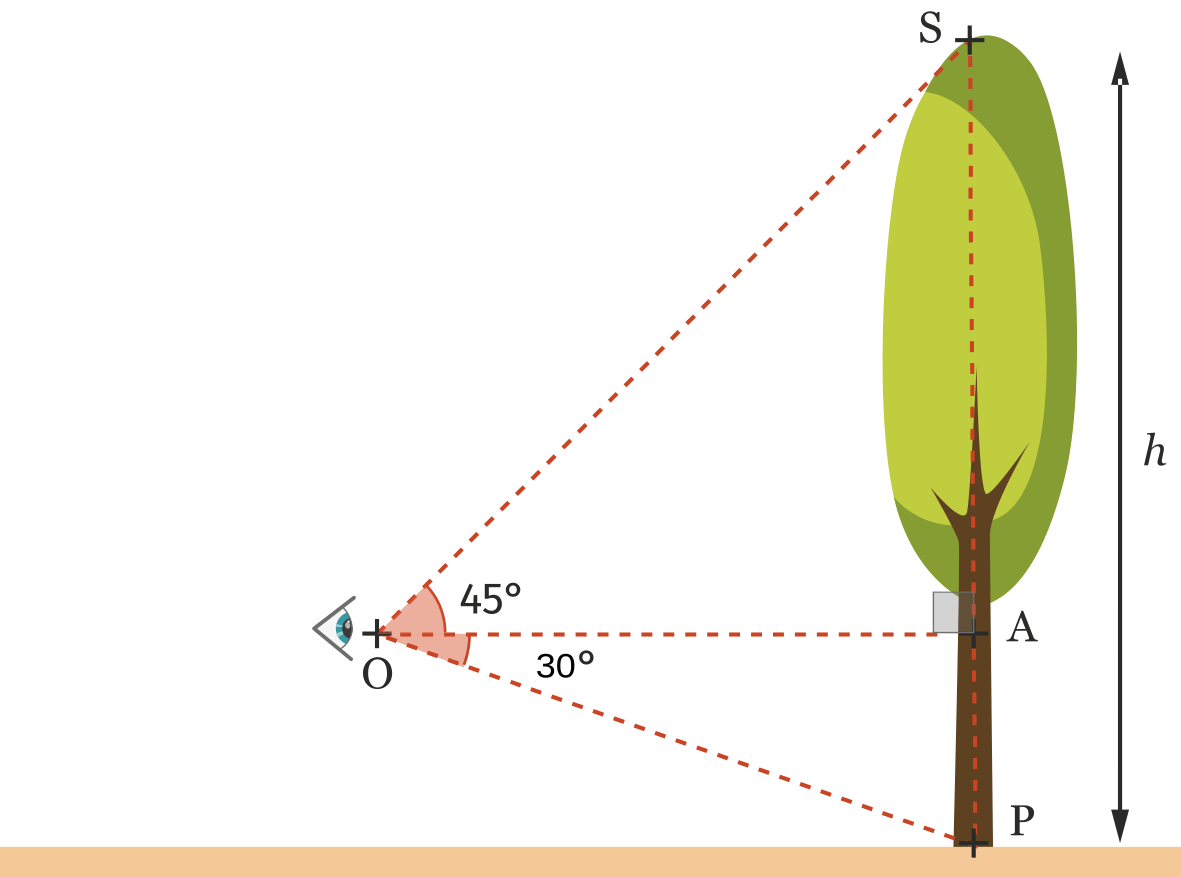
\includegraphics[width=8cm]{pin}
\end{minipage}



\exo{}
Pour fixer un éclairage sur la façade de sa maison, Jeanne doit poser une échelle contre le mur.\\
Pour qu'elle soit stable et pour éviter de glisser, cette dernière doit former un angle d'au moins 60° avec le sol. L'échelle mesure 2 m. Gênée par un bassin qui longe la maison, Jeanne n'a pu poser l'échelle qu'à 1,10 m du mur.\\[.5em]
Cette échelle sera-t-elle suffisamment stable?


\subsection*{Applications}

\begin{minipage}{8.5cm}
	\exo{}
	En physique, l'intensité du courant alternatif est donnée par la formule suivante : \\
	$\ i(t)=i_0\times \sin(\omega t+\phi)\quad$ où $\quad \omega=100\pi$ rad.s$^{-1}\quad$ et $\quad\phi$ représente le déphasage du signal.\\
	On a tracé ci-contre quatre fonctions représentant différentes intensités de courant alternatif pour lesquelles $\quad i_0=2$ A.
\end{minipage}
\begin{minipage}{8.5cm}
	\flushright 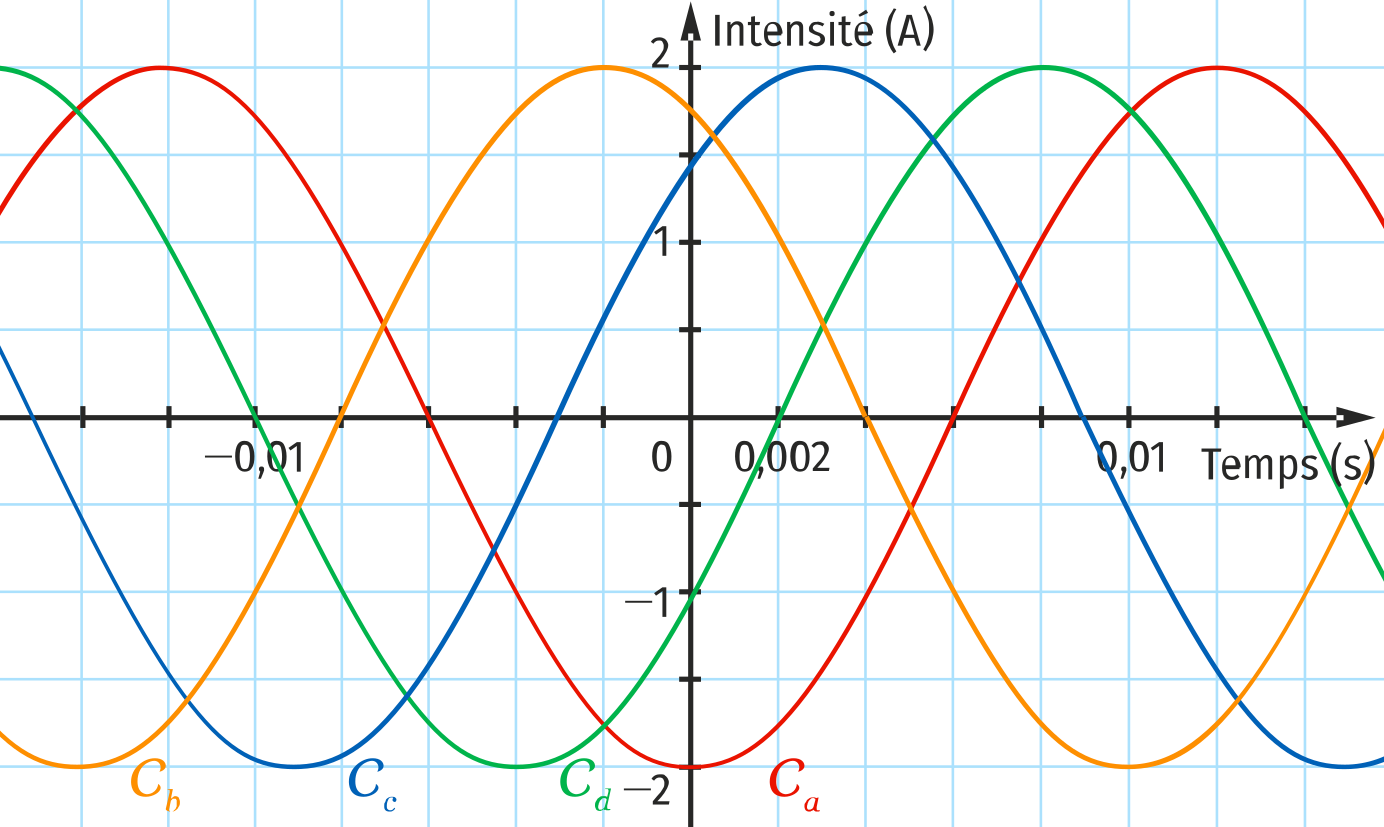
\includegraphics[width=8cm]{courbe1}
\end{minipage}
\begin{enumerate}
	\item 	Sans calculatrice, associer à chaque courbe l'expression ci-dessous qui lui est associée.
	\begin{multicols}{2}
		\begin{enumalph}
			\item 	$i_1(t)=2\sin\left(100\pi\times t+\dfrac{3\pi}{2}\right)$
			\item 	$i_2(t)=2\sin\left(100\pi\times t-\dfrac{\pi}{6}\right)$
			\item	$i_3(t)=2\sin\left(100\pi\times t+\dfrac{\pi}{4}\right)$
			\item	$i_4(t)=2\sin\left(100\pi\times t+\dfrac{2\pi}{3}\right)$
		\end{enumalph}
	\end{multicols}
	\item 	Deux signaux $S$ et $S'$ sont dits de même amplitude mais en opposition de phase si $i_0=i'_0$ et $\phi-\phi'=\pi$ ou $\phi-\phi'=\pi$.\\
	\begin{minipage}{8cm}
		\begin{enumalph}
			\item 	Montrer que les signaux d'intensité\\
			$i_5(t)=2\sin\left(100\pi\times t-\dfrac{\pi}{2}\right)$ et \\
			$i_6(t)=2\sin\left(100\pi\times t+\dfrac{\pi}{2}\right)$ sont de même amplitude mais en opposition de phase.
			\item 	 On a représenté, ci-contre, l'intensité des deux signaux précédents.\\
			Conjecturer la somme de leurs intensités.
		\end{enumalph}
	\end{minipage}
	\begin{minipage}{8.5cm}
		\flushright 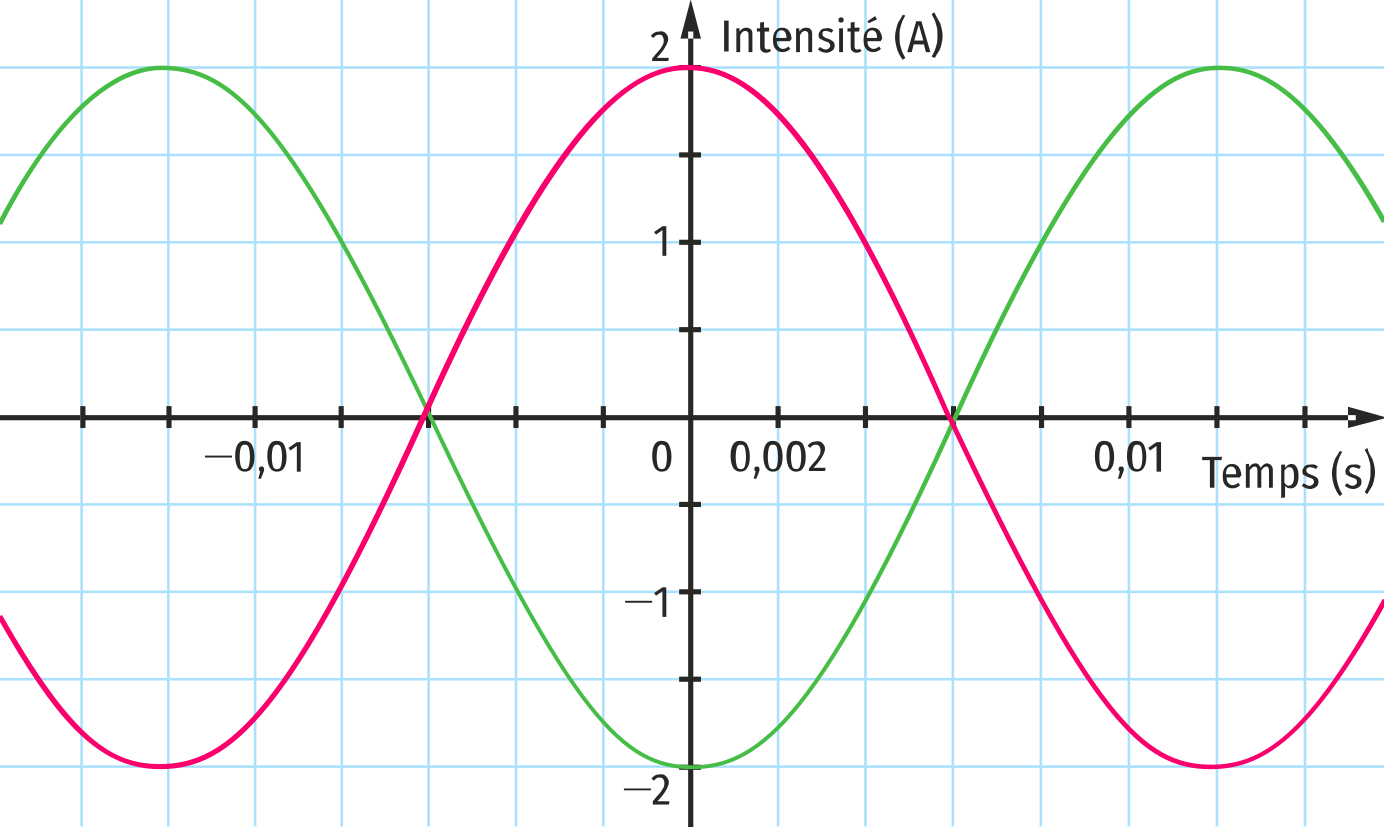
\includegraphics[width=8cm]{courbe2}
	\end{minipage}
\end{enumerate}



\exo{}
\begin{minipage}{9.5cm}
	
	On considère le triangle $ABC$ ci-contre.\\
	Avec les notations da la figure, on admet la formule suivante appelée la loi des sinus :
	$$\dfrac{a}{\sin(\alpha)}=\dfrac{b}{\sin(\beta)}=\dfrac{c}{\sin(\gamma)}.$$
	On appelle $S$ l'aire du triangle $ABC$.
\end{minipage}
\begin{minipage}{7.5cm}
	\flushright 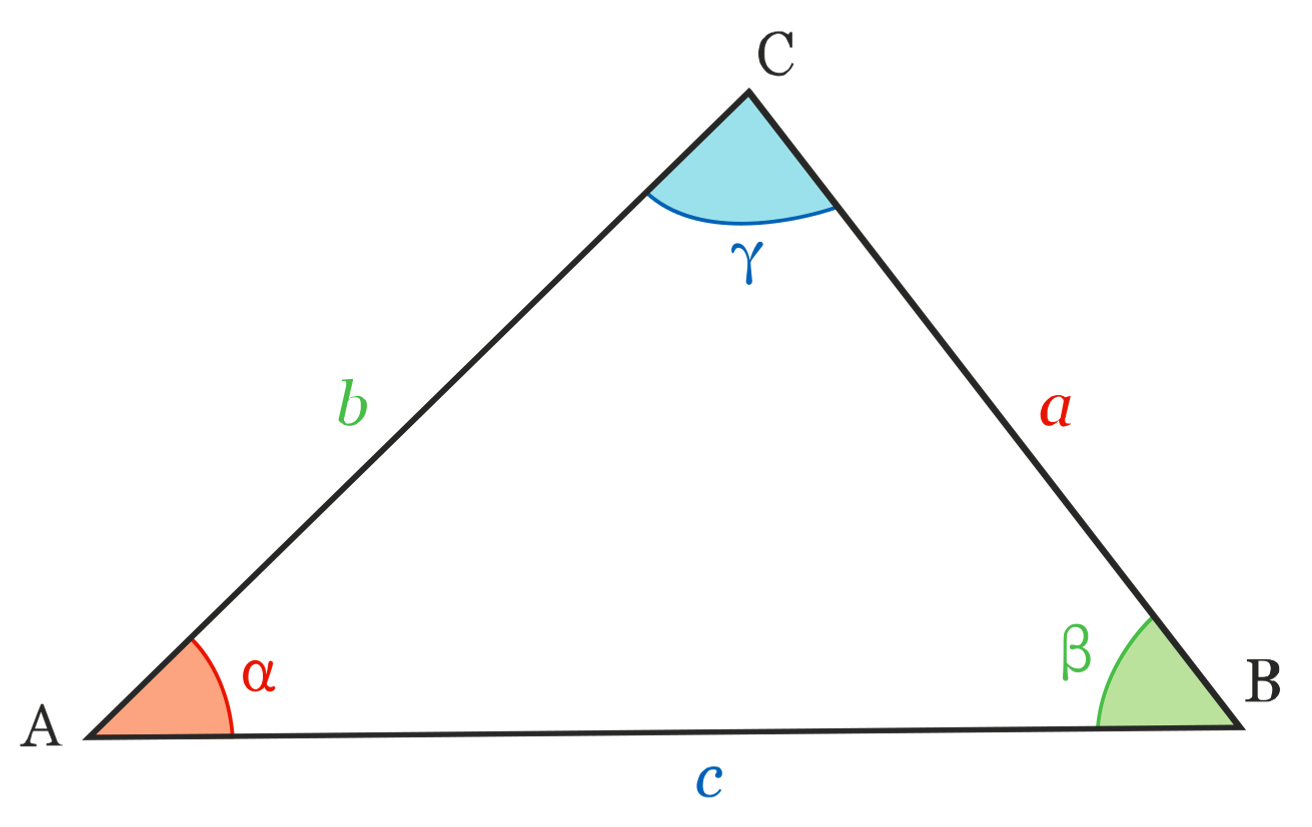
\includegraphics[width=7.5cm]{triangle}
\end{minipage}
\begin{enumerate}
	\item 	Montrer que : $\quad \dfrac{a}{\sin(\alpha)}=\dfrac{b}{\sin(\beta)}=\dfrac{c}{\sin(\gamma)}=\dfrac{abc}{2S}.\quad$
	\textit{On pourra utiliser une hauteur du triangle.}
	\item 	On suppose que : $\quad a=4$ cm, $c=7$ cm et $\beta=60°.\quad$	Déterminer la valeur de $S$.	
	\item	\textbf{Question bonus :} Démontrer la loi des sinus dans le triangle $ABC$.\\
	\textit{Indication : on pourra exprimer l'aire de $ABC$ de trois manières différentes.} 
\end{enumerate}


\begin{minipage}{9cm}
	\exo{}
	Un ornithologue souhaite connaître la distance parcourue par les hirondelles lorsqu'elle migrent de Bordeaux vers Libreville, au Gabon, au mois de septembre.\\
	Ce chemin est modélisé par la ligne rouge qui correspond à un arc de grand cercle sur la sphère terrestre.\\
	On sait que le rayon de la Terre est de 6371 km.\\[.5em]
	Déterminer la longueur de leur trajet au kilomètre près.
\end{minipage}
\begin{minipage}{8cm}
	\flushright 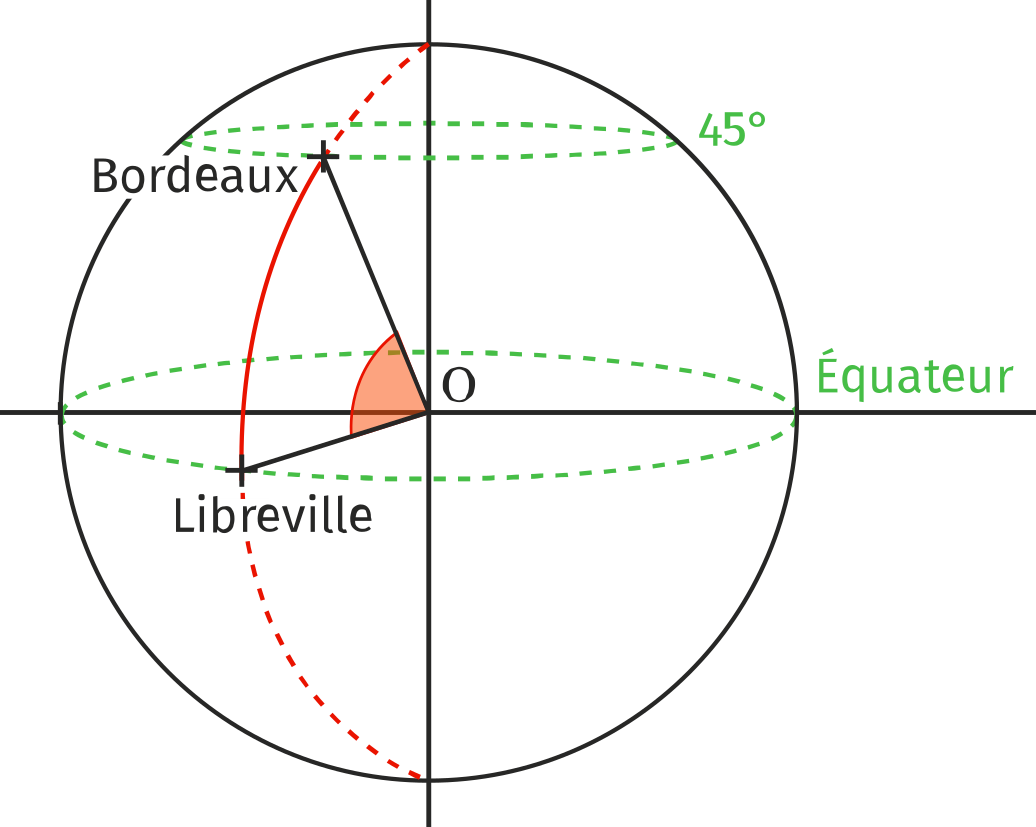
\includegraphics[width=7.5cm]{sphere}
\end{minipage}

\vspace{.5cm}


\begin{minipage}{8.5cm}
	\exo{}
	Un héron repère un poisson dans l'eau. Il souhaite plonger pour l'attraper, mais il sait que lorsque la lumière passe d'un milieu à l'autre, elle subit une déviation. Il ne doit donc pas aller « tout droit ».\\[1em]
	Déterminer, au degré près, la valeur de l'angle $\alpha$ ($\alpha=\widehat{BCA}$) pour que son plongeon lui permette d'attraper réellement sa proie (en supposant qu'il aille en ligne droite).
\end{minipage}
\begin{minipage}{8.5cm}
	\flushright 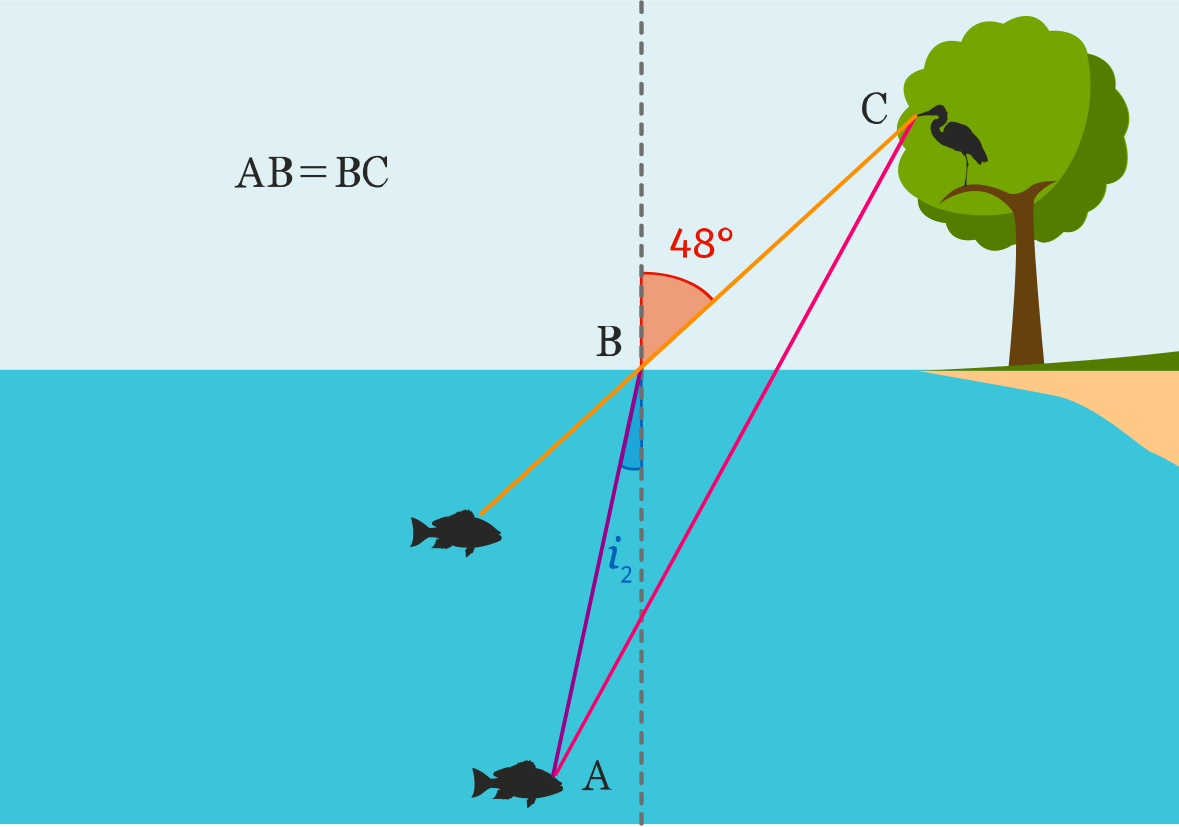
\includegraphics[width=8cm]{heron}
\end{minipage}

\begin{encadrecolore}{Rappel du cours de physique de \seconde}{UGLiOrange}
	\begin{minipage}{10cm}
		Lorsqu'un rayon issu d'un milieu d'indice $n_1$ se réfracte dans un milieu d'indice $n_2$ en formant des angles respectivement $i_1$ et $i_2$, alors ils sont liés par la formule : $$ n_1\times \sin(i_1)=n_2\sin(i_2)$$
		Pour l'eau et l'air, on a : $\ n_{eau}=1,33\ $ et $\ n_{air}=1$.
	\end{minipage}
\begin{minipage}{6.5cm}
	\flushright 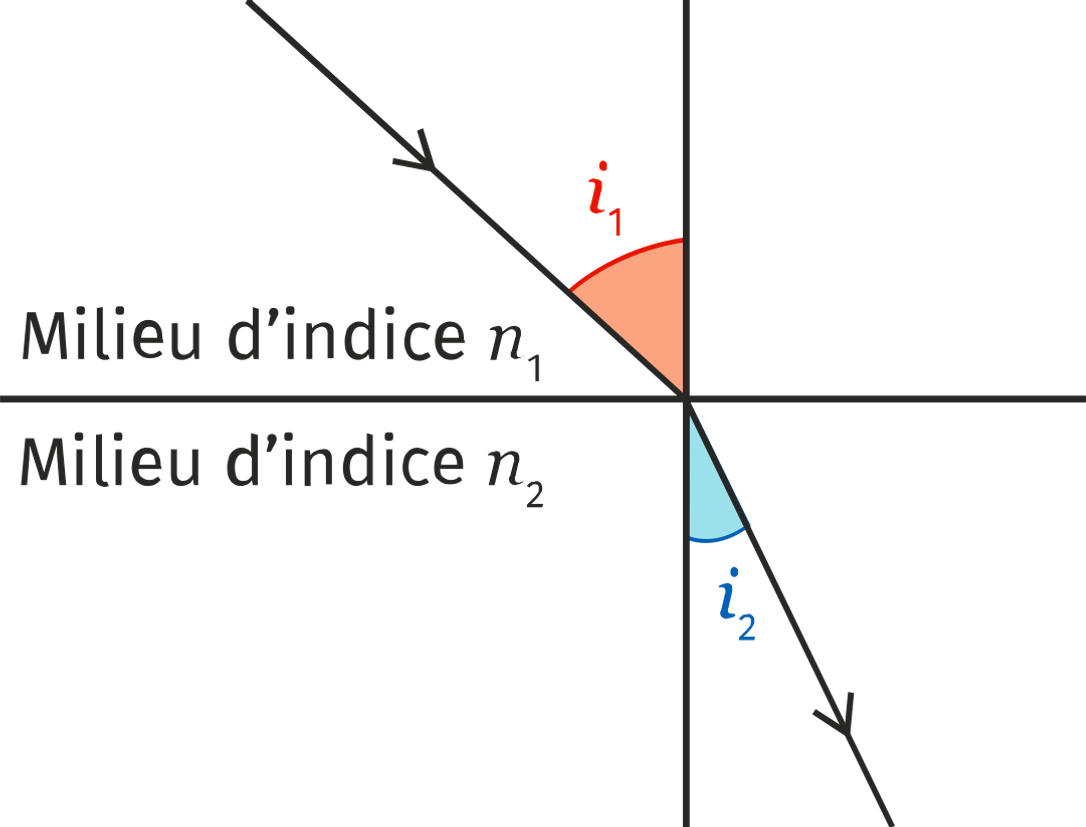
\includegraphics[width=6cm]{SnellDescartes}
\end{minipage}
\end{encadrecolore}



\exo{ \'Equations trigonométriques}
Résoudre les équations suivantes :
\begin{multicols}{2}
	\begin{enumerate}
		\item 	$\sqrt{2}\cos x +1 = 0$ dans $\oio{-\pi}{\pi}$.
		\item 	$2\cos^2x-9\cos x+4=0$ dans $]-\pi;\pi[$.
		\item 	$\sin\left(x+\dfrac{\pi}{4}\right)=\dfrac{1}{2}$ dans $\fio{0}{2\pi}$.
		\item 	$2\sin^2x-3\sin x+2=0$ dans $\fio{2\pi}{4\pi}$.
		\item 	$2\cos^2x+15\cos x+7=0$ dans $\oif{-\pi}{\pi}$.
		\item  	$2\sin^2x-3\cos x-2=0$ dans $\oif{-\pi}{\pi}$.
		\item 	$4\sin^2x-3=0$ dans $]-\pi;\pi]$.
		\item 	$\bigstar$\ Résoudre dans $]-\pi;\pi[$ : $\quad\sin3x=\dfrac{1}{2}$.	
	\end{enumerate}
\end{multicols}

\end{document}
